\chapter{Implementation Details}
In this chapter a more in depth explanation of the implementation of the project will be provided. The operations of generating the PUFs and applying a challenge are done in part on the host side and in part on the board side.

The Host is responsible of communicating to the board what operation must be done, by sending command codes, and getting back the results. Also the Host is the one that will have access to the PUF database.
The Board is responsible to perform the hashing of the PUFs and provide access to the SRAM, where the PUFs will be stored.

The host will ask from the board to perform two operations
\begin{itemize}
	\item Get the PUFs and store them in the DB of PUFs.
	\item Once a challenge is provided, access the DB and get the PUF. Then pass the challenge and the expected result to the board which will compare it to the PUF that is stored in memory.
\end{itemize}

The operations that the board must be able to perform are three:
\begin{itemize}
	\item Read the PUFs from the RAM and store them in the SRAM. This must be done as soon as the device is powered on.
	\item Read the PUFs from the SRAM, hash them and send them back to the host
	\item Once the challenge is provided read the PUF from the SRAM, compute the hash and compare it to the hashed PUF given by the host.
\end{itemize}

 possible two files had to be changed
\begin{enumerate}
	\item $USBStick > Startup > startup\_stm32f429nihx.s$
	\item $USBStick > Src > Device > se3\_dispatcher\_core.c$
\end{enumerate}

\section {PUF retrieval and DB initialization}

At the beginning it is necessary to access the RAM at the correct time and copy the values found in the SRAM so that they can be read later on. Once we can read them we store them so that later on we can refer to them as the PUFs that can identify the device. To perform this operation we have some things to be done on both host and board side.

\subsection{Host side}

To get the correct data from the RAM that represent the PUFs it is necessary to access the memory immediately after the board startup and before writing any data to the SRAM. This means that an erase of the memory must happen and data must be overwritten. So before using the functions a board initialization is performed.

Once this is done the host works in two stages. One to access the DB and one to prepare the parameters to be send to the board.

For the DB initialization, which is done in the $examples > puf\_db\_init.cpp$, we don't need to send any parameters, except for the pointer to the returned data.
The actual communication with the board is done through the use of functions implemented in the L1\_security library. In that library we have provided the $L1GetPUFS$ function that is responsible of transmitting the parameters to the board and receiving the results from the board.

\begin{figure}[h!]
	\vspace{0.5cm}
	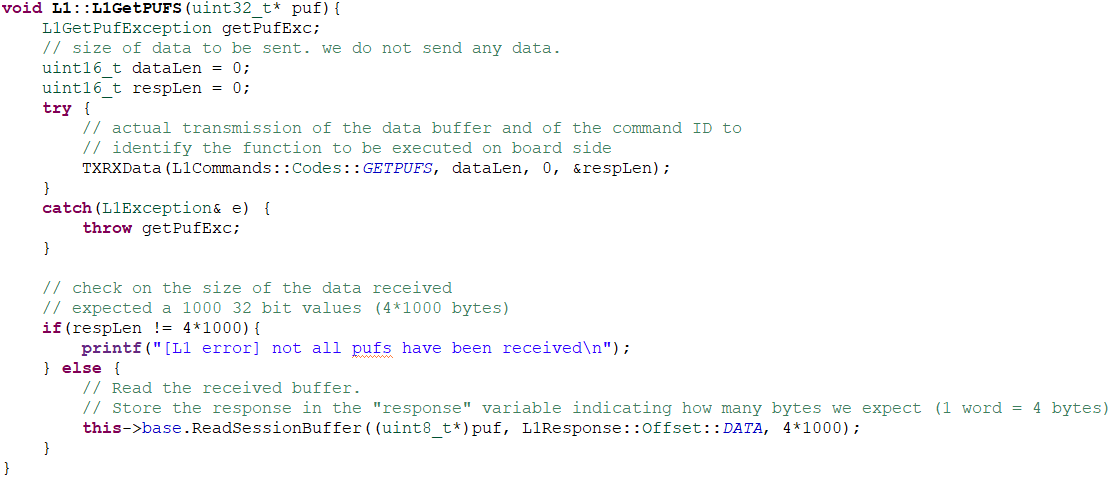
\includegraphics[width = 0.8\textwidth]{images/L1GetPUFS.png}
	\caption{Function responsible for communicating with the board. }
	\label{fig:L1GetPUFS}
\end{figure}

In that piece of code we can see that we are expecting 1000 PUFS but byte since the TXRX function works in bytes. In that operation we must provide the size of the data we are transmitting/receiving and also the ID of the command to execute on the board side.
The host is then responsible then to write that data to the DB.

\subsection{Board side}

In this stage the board is responsible of retreiving the initial data, PUFs, from the RAM and store them to the SRAM so that they can be accessed safely later.

Since the the content of the RAM will be overwritten the PUFs must be copied as soon as possible. For this reason this operation has to be done before any memory initialization. So this operation is done in the startup assembly file in which the reset handler can be found. This way we guarantee that we read the RAM before any memory initialization.

Since the the flash memory needs control registers to be accessed safely we relied on the HAL functions. More precisely the functions to unlock and program/write in memory. The code written to perform this operation is provided in figure \ref{fig:code_assembly}

\begin{figure}[h!]
	\vspace{0.5cm}
	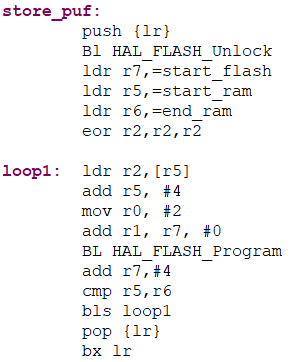
\includegraphics[width = 0.3\textwidth]{images/code_assembly.png}
	\caption{Assembly code to store PUFs into the flash memory. }
	\label{fig:code_assembly}
\end{figure}

Using the reference manual for the MCU (STM32f429) we know the memory mapping of both the SRAM(0x020000000 -  0x02002FFFF) and flash memory(0x08000000 - 0x081FFFFF). Starting from that we scanned the SRAM and loaded the content to a part of the flash memory that will not compromise sensible data.

At the end of the execution of the assembly code we expect 1000 PUFs to be stored in the flash memory which will be accessible once we enter the main and the execution loop where we can call implemented functions and access the content of the SRAM.

Once we have the PUFs in memory we need to able to access them. This is done through the $puf\_retreive()$ function, found in the $se3\_dispatcher\_core.c$ file. This is the function associated to the command code transmitted on the Host side.

To make the command call possible it is necessary to define these commands in the $se3\_dispatcher\_core.h$ which must reflect the number associated to the same also on the host side.

\begin{figure}[h!]
	\vspace{0.5cm}
	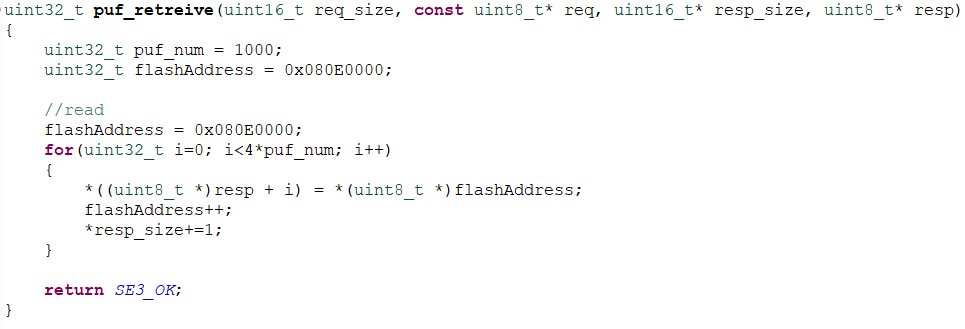
\includegraphics[width = 0.8\textwidth]{images/puf_retreive().png}
	\caption{puf\_retreive function. }
	\label{fig:puf_retreive}
\end{figure}

In this function we simply read from the SRAM the PUFS that we stored in the assembly code. This data is the data that will be sent to the host side, as parameter resp, once they have been hashed. 


\section {Application of a challenge and verification of the device} 
\label{section:impl_host}

Once we have the DB filled with the PUFs we can use that to check the authenticity of the board by comparing the PUFs in the DB and the ones regenerated by the board. Again to realize the functionality we will have to do some things on the host and some on the board side.

\subsection{Host side}

The approach is similar to the one used for reading the PUFs but now we have different parameters to transmit. In fact we need to provide both the challenge and the PUF read from the DB. So the Host is responsible of getting the challenge, use it to access the DB and retrieve the response PUF. From there a compaction of both parameters into one is done so that they can be sent as one parameter to the board. These operations are done in the $examples > puf\_challenge.cpp$ file shown in figure \ref{fig:puf_challenge.cpp}

\begin{figure}[h!]
	\vspace{0.5cm}
	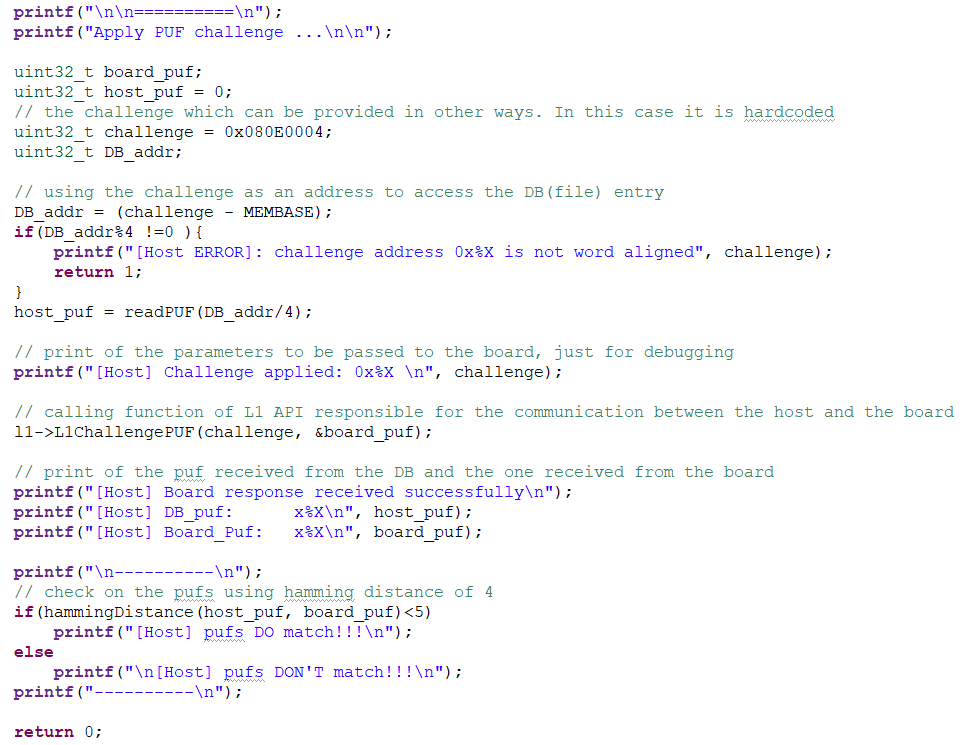
\includegraphics[width = 0.8\textwidth]{images/puf_challenge.png}
	\caption{puf\_challenge.cpp}
	\label{fig:puf_challenge.cpp}
\end{figure}

Then the next stage is to perform the actual transmit/receive done in the L1\_security library in the L1ChallengePUF function, shown in figure \ref{fig:L1ChallengePUF}.

\begin{figure}[h!]
	\vspace{0.5cm}
	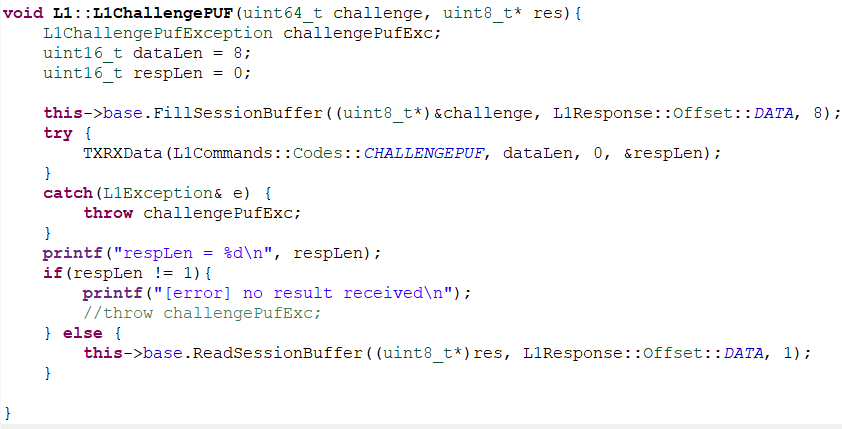
\includegraphics[width = 0.8\textwidth]{images/L1ChallengePUF.png}
	\caption{L1ChallengePUF function for transmitting challenge and response PUF}
	\label{fig:L1ChallengePUF}
\end{figure}

In this function we have some data to transmit and since the TXRX works with bytes we have to indicate the size in bytes which is 8 since we transmit 32bit challenge and 32bit PUF. Then as response we expect just one byte to indicate match found (1) or match not found (0).

\subsection{Board side}

The Board at this point has been provided with the challenge and the PUF to use as reference.

The first operation to be done is to extract the compacted data received and obtain again the challenge and the PUF. In doing so we must be aware of the endianness used. From there we can access the SRAM using the challenge as an address and the content must be the PUF.

Since the PUF read from the DB is hashed the board must also perform a hashing on the PUF read from the memory before comparing it to the one from th DB, the result of which will be sent back and evaluated by the Host.

\begin{figure}[h!]
	\vspace{0.5cm}
	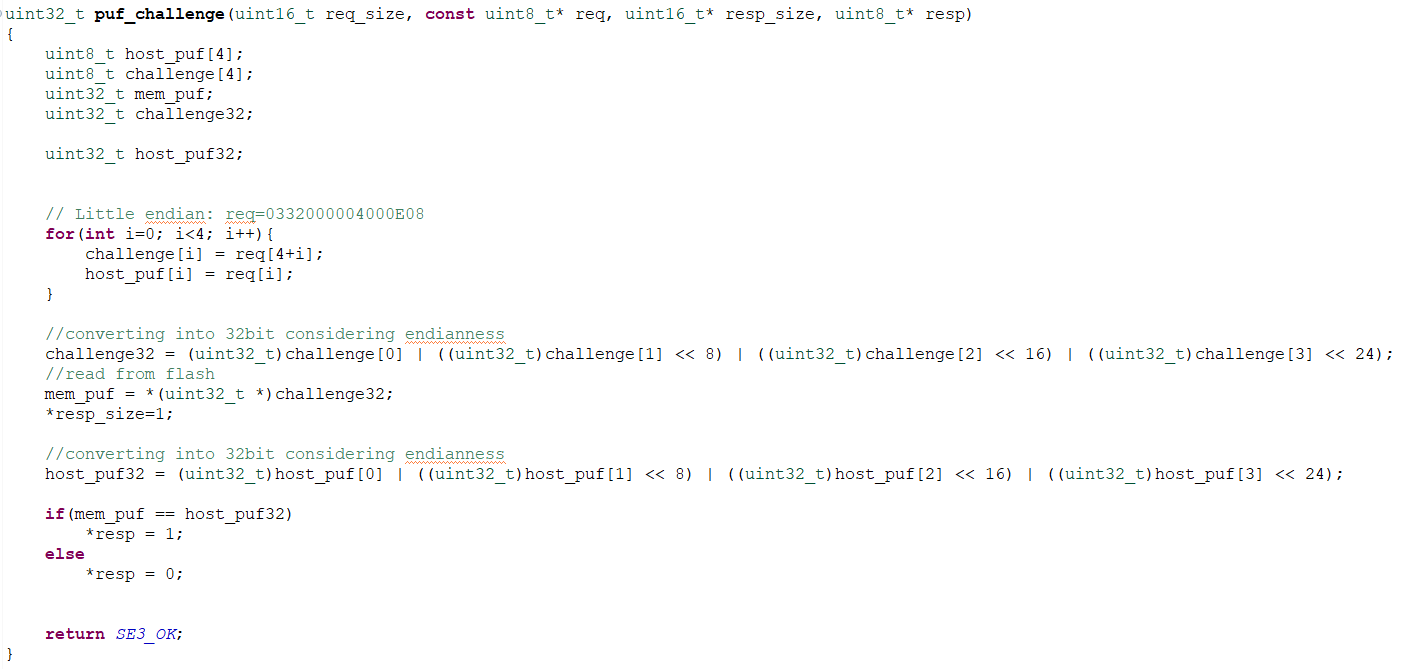
\includegraphics[width = 0.8\textwidth]{images/puf_challenge_board.png}
	\caption{puf\_challenge\_board function on the board side}
	\label{fig:puf_challenge_board}
\end{figure}
